\documentclass[../main.tex]{subfiles}

\begin{document}
\section{Características técnicas de los modelos a implementar}
\subsection{Cycle GAN}

En primer lugar, una vez explicado el concepto de Cycle GAN en la sección \ref{Cycle GAN}, tenemos que mencionar las arquitecturas de las redes discriminadoras y generadoras que vamos a implementar. En el paper original \cite{Zhu2017} se proponen dos arquitecturas diferentes para el generador (U-Net y ResNet) y una para el discriminador (PatchGAN). Explicamos el fundamento de cada una a continuación.

\subsubsection{U-Net}

Como puede apreciar el lector en la figura \ref{fig:unet}, el nombre de red u no es casualidad. 

\begin{figure}[h]
    \centering
    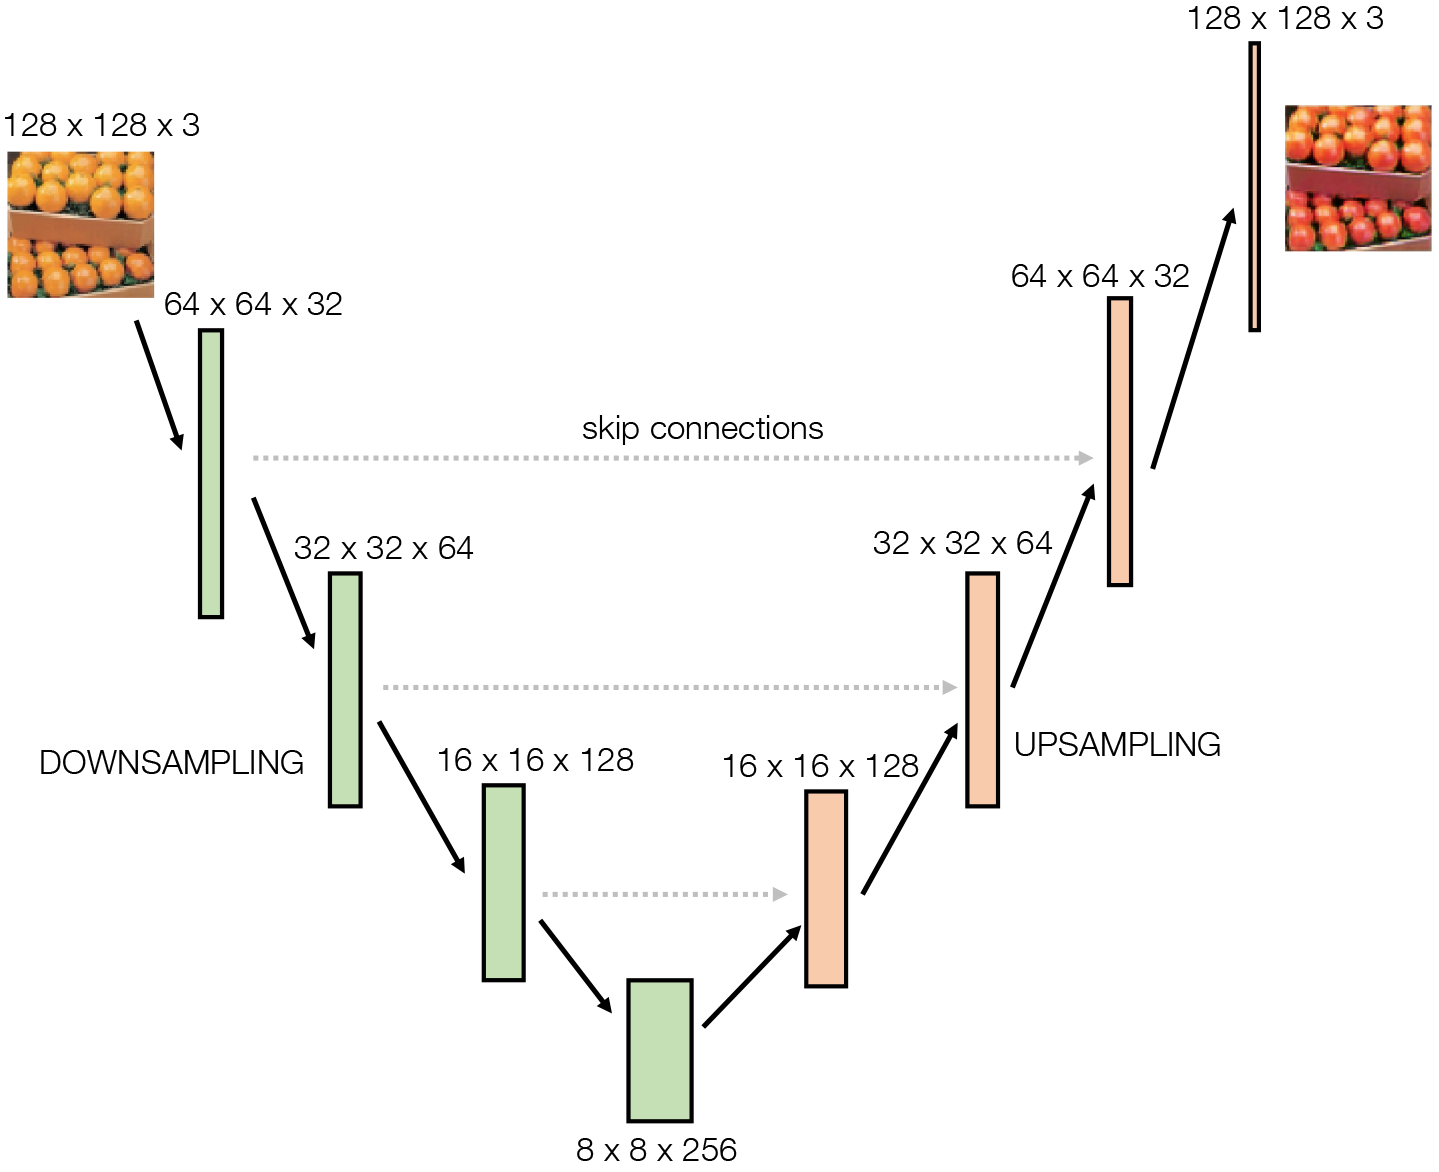
\includegraphics[width=0.8\textwidth]{imagenes/unet.png}
    \caption[Arquitectura U-net]{Arquitectura U-net. Extraido de \cite{Foster2019}}
    \label{fig:unet}
\end{figure}

En la primera mitad de la U se realizan operaciones en las que se reduce la imagen (\textit{downsampling})  espacialmente pero se aumenta su número de canales y la segunda parte, la cual realiza la operación contraria (\textit{upsampling}): aumenta la resolución espacial pero reduce el número de canales. No obstante, el flujo de la imagen es lineal: tenemos \textit{atajos} o \textit{skip connections} que comunican dos capas no contiguas, lo que permite disponer de más información en las capas de aumento. \newline

Esta arquitectura sintetiza lo siguiente: las operaciones de reducción reconocen lo que hay en la imagen pero no aportan información sobre dónde está lo que reconocen. En el vértice de la U se conoce qué es lo que hay en la fotografía, pero no de su localización espacial; por lo que si simplemente quisiéramos realizar segmentación de la imagen ya habríamos acabado. \newline

Como no queremos únicamente segmentar la imagen, al ampliar la resolución (segunda parte de la U) tenemos que \textit{indicar} a la capa dónde tiene que buscar lo que ya sabe. Esta información es aportada mediante los \textit{atajos}, lo que nos permite combinar la información relacionada con el \textit{qué hay} en la imagen junto con el \textit{dónde está} \cite{Ronneberger2015} \cite{Foster2019}.

\subsubsection{ResNet}

Esta arquitectura es bastante parecida en concepto a la anterior, ya que también permite el paso de información entre capas no continuas a través de \textit{atajos}; pero su implementación es diferente: en lugar de realizar una U para conseguir esos \textit{atajos}, se aplana esa U (pasando a un flujo complemtamente lineal) y se realizan menos operaciones de aumento y reducción; pero colocando entre medias bloques residuales (de ahí el Res del nombre). La figura \ref{fig:resnet} muestra la arquitectura resnet.

\begin{figure}[h]
    \centering
    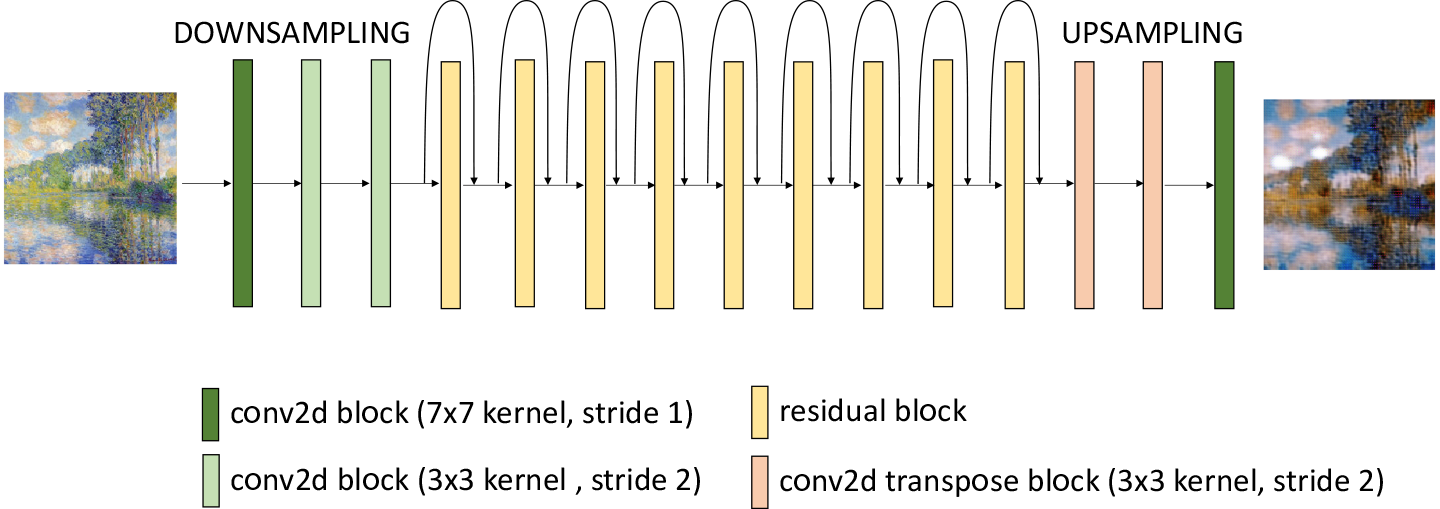
\includegraphics[width=0.8\textwidth]{imagenes/resnet.png}
    \caption[Arquitectura resnet]{Arquitectura resnet. Extraido de \cite{Foster2019}}
    \label{fig:resnet}
\end{figure}

Esos bloques residuales disponen de un \textit{atajo}, permitiendo sumar al final del bloque los datos que ya teníamos en la entrada junto con el resultado de la capa actual. La figura \ref{fig:bloque_residual} lo muestra gráficamente \cite{He2016} \cite{Foster2019}. 

\begin{figure}[h]
    \centering
    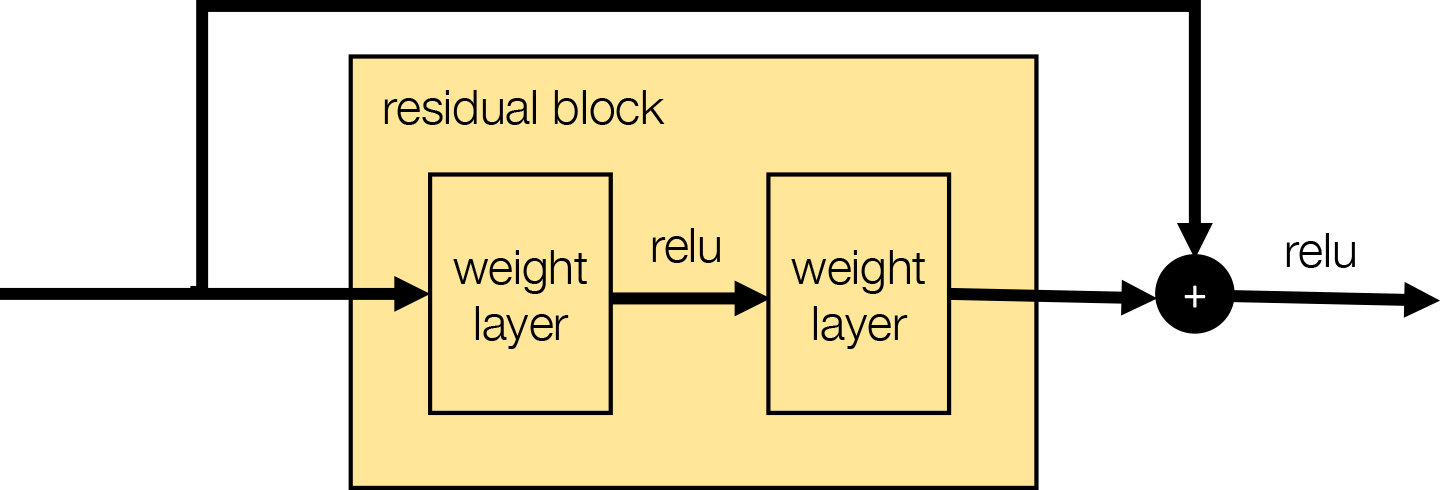
\includegraphics[width=0.75\textwidth]{imagenes/bloque_resnet.png}
    \caption[Bloque resnet]{Bloque resnet. Extraido de \cite{Foster2019}}
    \label{fig:bloque_residual}
\end{figure}

La utilidad de esta arquitectura es que permite añadir cientos y miles de capas sin sufrir el problema de desvanecimiento de gradiente \footnote{En algunos casos, el gradiente de la función error tiende a valores muy pequeños, lo que en los peores casos impide que la red continué aprendiendo debido a que se queda \textit{atascada}, recibiendo únicamente actualizaciones de sus pesos con valor 0.}. Asimismo, se cree que añadiendo capas adicionales los resultados serán como mínimo igual de buenos, ya que si la capa añadida no es capaz de extraer información relevante, al sumar los resultados con los de la entrada del bloque residual seguimos conservando los datos pre-capa.

\subsubsection{PatchGAN}

Este discriminador, heredado de la red homónima, parte de una idea bastante sencilla de comprender \cite{Foster2019}: en lugar de tener un discriminador que evalúa la imagen por completo y tiene por salida un número que indica la probabilidad de que la imagen de entrada sea \textit{real}; PatchGAN propone un discriminador \cite{Assens} (basado en la red convolucional VGG16 \cite{Neurohive2018}) que proporciona una salida tensorial de 8x8 (calculado en paralelo) en lugar de un solo número. Ese 8x8 corresponde a que la imagen se divide en ese número de secciones, siendo cada escalar del tensor la probabilidad estimada de ese trozo de imagen. \newline

Este enfoque permite que la función pérdida puede centrarse el estilo de la imagen (presente en cada sección de la imagen) en lugar del contenido (disperso a lo largo de las subimágenes), es decir, forzamos al discriminador a tener que fijarse en el estilo y no en los elementos de la imagen, que es lo que queremos discriminar en este problema.

\subsection{Méticas de la CycleGAN}

Como en cualquier modelo de redes neuronales la función pérdida es muy importante. Sin profundizar en las expresiones matemáticas, el modelo CycleGAN establece tres criterios diferentes:

\begin{enumerate}
    \item Validez: ¿las imágenes creadas por cada generador engañan al discriminador correspondiente? Necesitamos que en este baremo el modelo lo haga realmente bien.
    
    \item Reconstrucción: si pasamos por un generador y luego el otro (en ambos sentidos), es decir, realizamos un ciclo por la red, ¿tenemos la imagen original? Aquí necesitamos que el error sea mínimo.
    
    \item Identidad: ¿si al generador le pasamos una imagen del mismo dominio (es decir, tenemos que el dominio origen y destino es el mismo), tenemos la imagen original? Nuevamente buscamos que este error sea lo más pequeño posible.
\end{enumerate}

\begin{figure}[h]
    \centering
    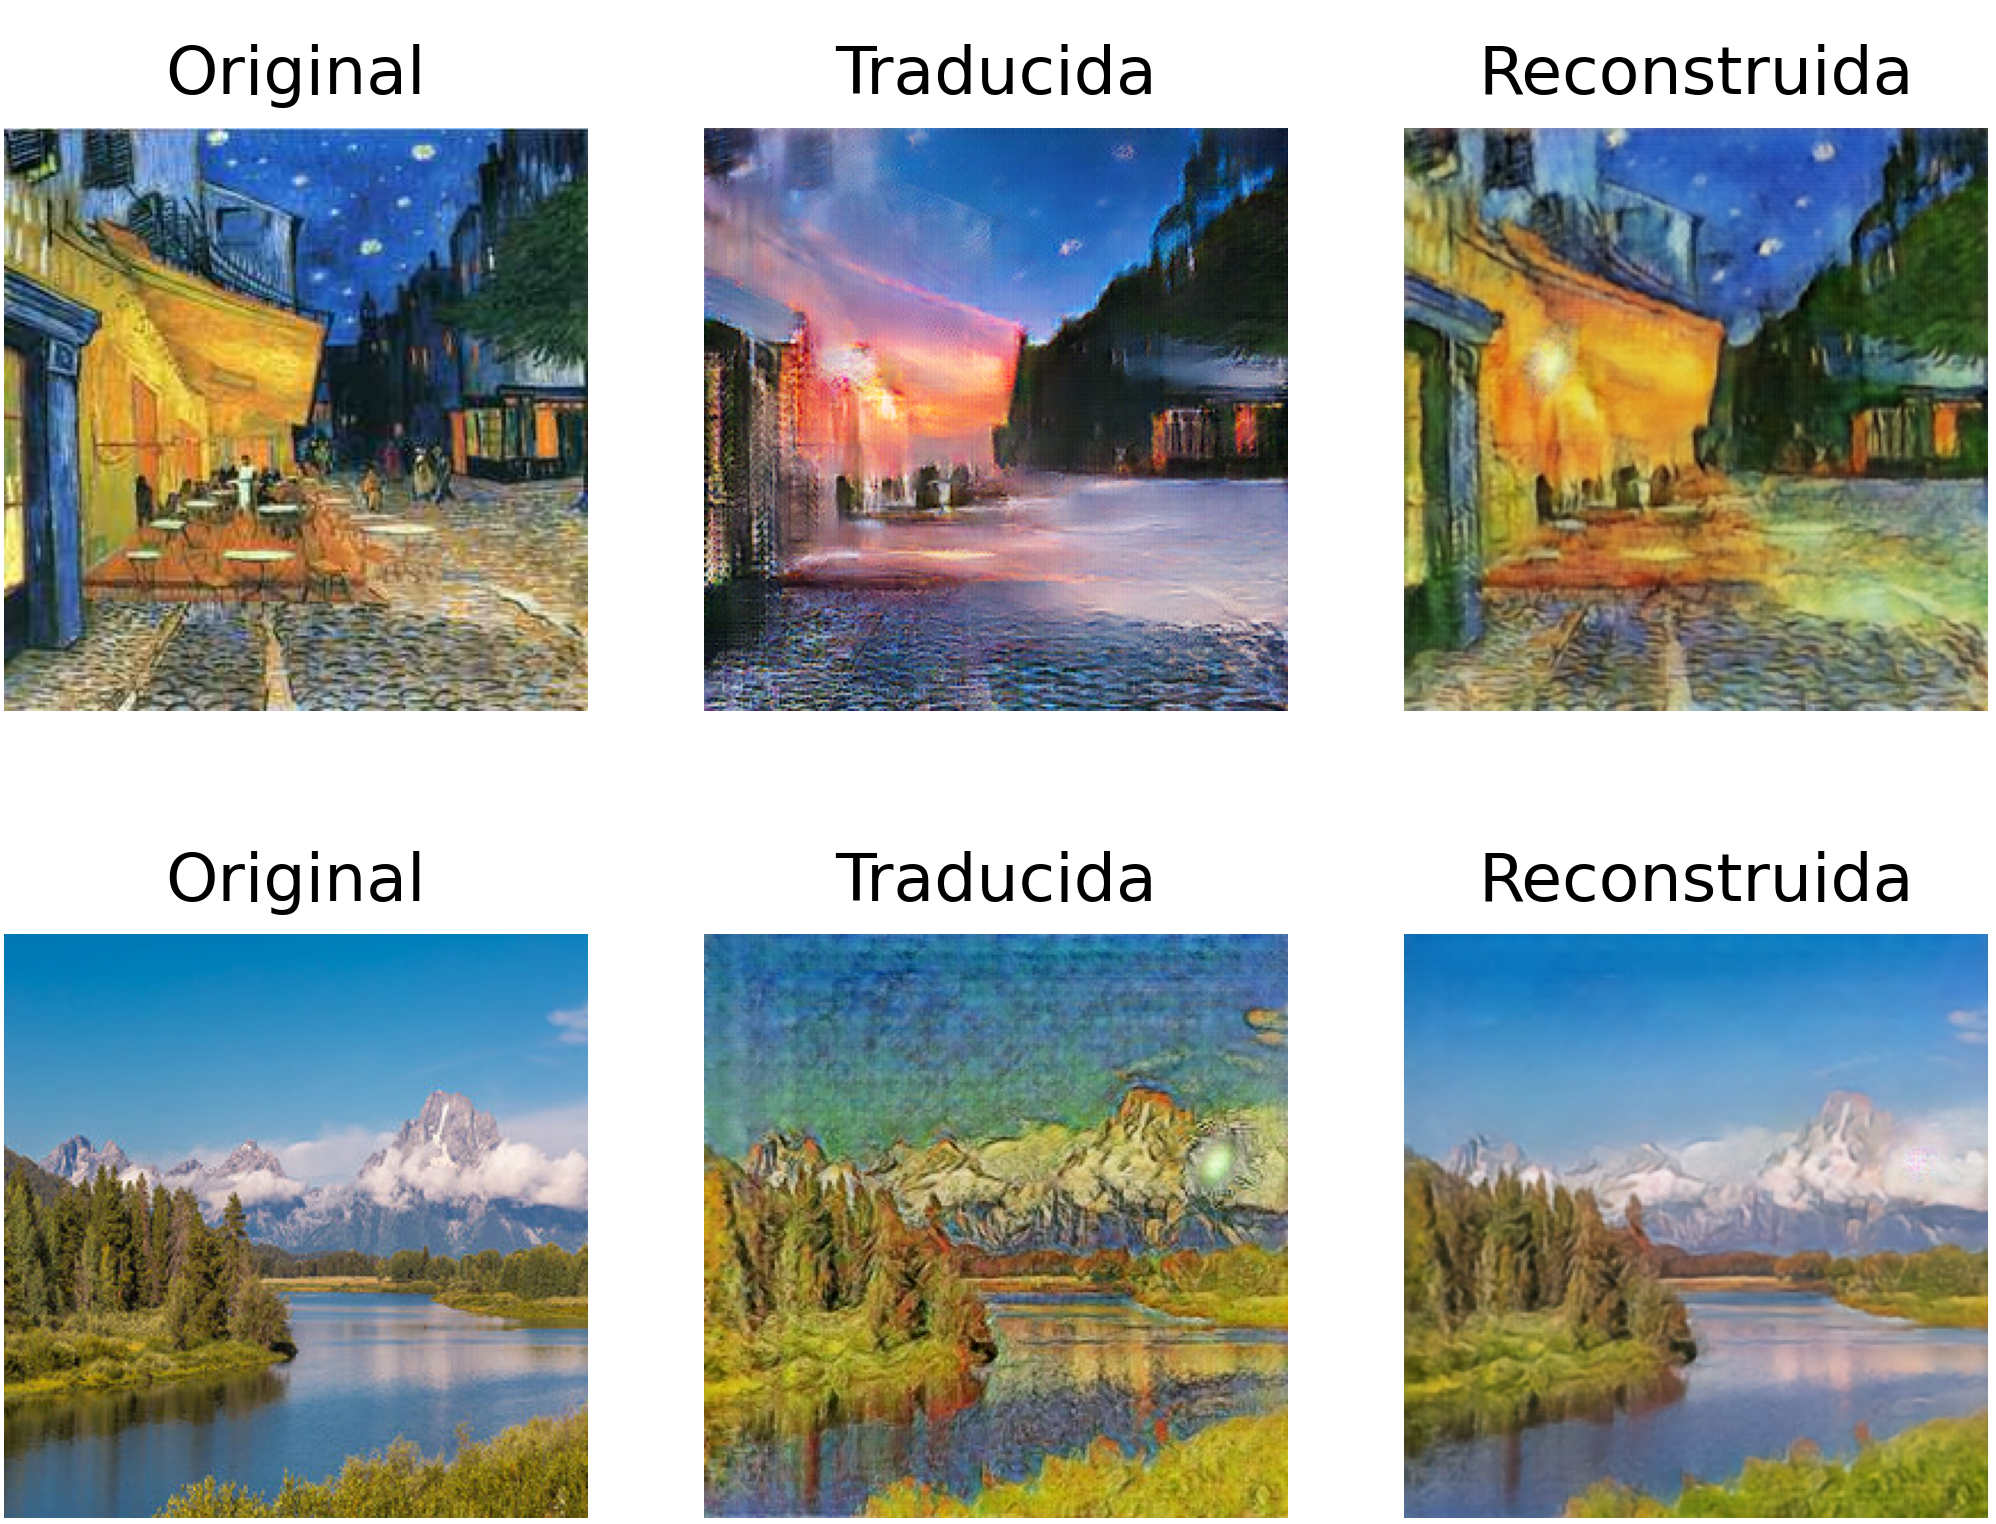
\includegraphics[width=0.8\textwidth]{imagenes/ciclo medidas cyclegan tensorboard.png}
    \caption[Medidas de validez y reconstrucción]{Medidas de validez y reconstrucción de la implementación con el dataset \textit{vangogh2photo}, ofrecidas por Tensorboard}
    \label{fig:ciclo_imagen_tensorboard}
\end{figure}

Las medidas de validez y reconstrucción suenan muy lógicas: una es el objetivo de la red y la otra asegura que los dos sentidos funcionen correctamente, pero la medida de identidad puede parecer poco importante. Para demostrar su importancia recurrimos al ejemplo mostrado en \cite{Foster2019}: si prescindimos del baremo identidad, vemos que se modifica la superficie de las frutas. Esa es la labor de la métrica de identidad: forzar al sistema que sólo modifique las partes de la imagen que son necesarias para la transformación. Sin embargo, las tres partes de la función error tienen que estar balanceadas: si la parte identidad tiene poco peso tendremos el fenómeno visto en el ejemplo, pero si es demasiado el sistema está sentenciado a la inanición.

\begin{figure}[h]
    \centering
    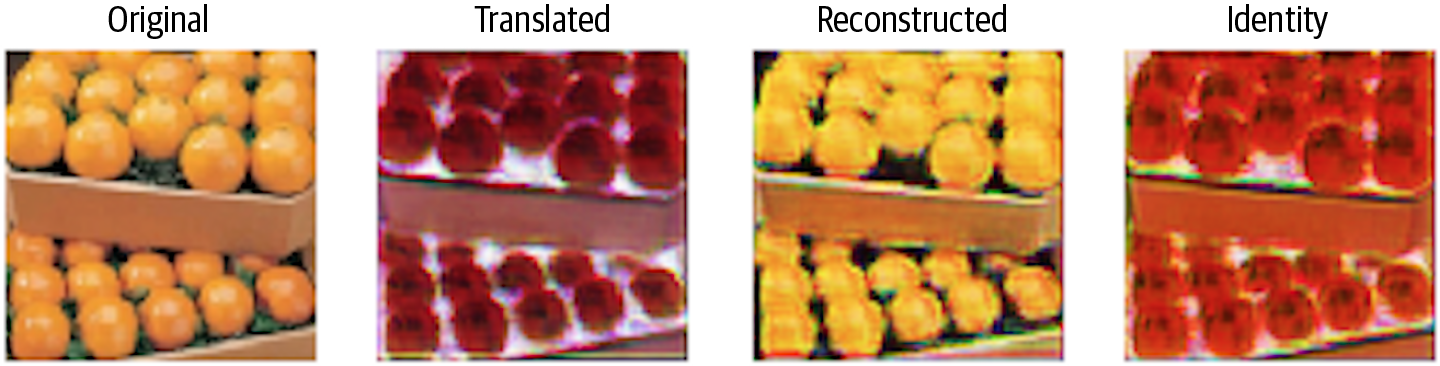
\includegraphics[width=1\textwidth]{imagenes/error_identidad_foster.png}
    \caption[Importancia del error identidad]{Importancia del error identidad. Tomado de \cite{Foster2019}.}
    \label{fig:error_identidad_foster}
\end{figure}

\subsection{EnhanceNet}

La red EnhanceNet es una red GAN diseñada para una tarea llamada súper resolución, que consiste en a partir de una imagen pequeña aumentarla de resolución sin que \textit{se vea pixelada} \cite{Sajjadi2016}. En este \tfg se utiliza esta red debido a las limitaciones que tiene CycleGAN con la resolución: con esta red podemos utilizar nuestra CycleGAN y posteriormente ampliar la resolución drásticamente para ofrecer imágenes de mayor calidad. \newline

\begin{figure}[h]
    \centering
    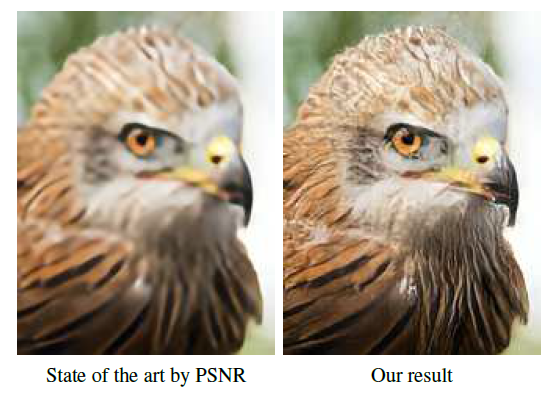
\includegraphics[width=0.65\textwidth]{imagenes/ejemplo_enhancenet.png}
    \caption[Ejemplo de EnhanceNet]{Ejemplo de EnhanceNet. Tomado de \cite{Sajjadi2016}.}
    \label{fig:ejemplo_enhancenet}
\end{figure}

EnhanceNet es una de las muchas redes que realizan esta tarea, pero la hemos elegido en este \tfg debido a que los autores tienen publicados los pesos de la red ya entrenada, lo que nos ahorra entrenar otra red desde 0. Asimismo esto nos permite tener un subsistema que amplíe la resolución de calidad y a coste 0, prescindiendo de servicios de pago. \newline

\begin{figure}[h]
    \centering
    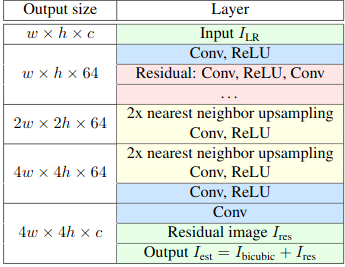
\includegraphics[width=0.55\textwidth]{imagenes/arquitectura_enhancenet.png}
    \caption[Arquitectura de EnhanceNet]{Arquitectura de EnhanceNet. Tomado de \cite{Sajjadi2016}.}
    \label{fig:arquitectura_enhancenet}
\end{figure}

Si bien no es necesario centrarnos en la red (en este trabajo se utiliza la red como una caja negra), en la figura \ref{fig:arquitectura_enhancenet} se describe la arquitectura de la red. Viendo la imagen vemos muchos nombres que nos resultan familiares: tenemos que EnhanceNet es una red convolucional que mediante bloques residuales aprende a ampliar las imágenes. Más concretamente, son 10 bloques residuales, lo que ayuda a que el modelo aprenda rápido \cite{Rapole2020}; además de utilizar una funcion de error (dentro de las cuatro que posee) inspirada en las redes CycleGAN. \newline

Por último, la red ofrece una \textit{imagen residual}, que es la diferencia entre la imagen deseada y la ampliación mediante un algoritmo conocido como interpolación bicúbica, el cual se detalla en \cite{Tabora2020}.

\section{Datos utilizados para elaborar el sistema}

Los datasets utilizados en este \tfg son tres: \textit{monet2photo}, \textit{vangogh2photo} y \textit{cezanne2photo}. Todos los datasets tienen la misma estructura: por un lado tenemos los cuadros del artista, mientras que por otro disponemos un conjunto de fotografías de paisajes. \newline

Dichos datasets fueron creados por los autores del paper del modelo CycleGAN \cite{Zhu2017}. De acuerdo con sus especificaciones, los autores descargaron las imágenes de los cuadros de la web \url{wikiart.org}, descartando los bocetos y las obras obscenas. Asimismo, las fotos fueron descargadas de \url{flickr.com} buscando por las etiquetas \textit{landscape} y \textit{landscapephotography}, obviando fotografías en blanco en negro. Todas las imágenes fueron redimensionadas a 256x256 pixeles. \newline

En total, se disponen de 1074 imágenes de Monet, 584 de Cézanne y 401 de Van Gogh, ya que los cuadros de Monet fueron filtrados para incluir únicamente cuadros de paisajes y sólo se incluyeron los trabajos finales de Van Gogh, buscando representar su estilo artístico más reconocible. \newline

Por otra parte, la estructura del cada dataset es la siguiente: se disponen de cuatro carpetas, llamadas \textit{trainA}, \textit{trainB}, \textit{testA} y \textit{testB}. Las carpetas con sufijo A contienen los cuadros, mientras que los que tienen sufijo B las fotografías. En las figuras \ref{fig:vista_previa_cuadros_cezanne} y \ref{fig:vista_previa_fotos_cezanne} mostramos una parte las carpetas \textit{trainA}, \textit{trainB} del dataset \textit{cezanne2photo}.

\begin{figure}[!htb]
  \begin{subfigure}[b]{0.49\textwidth}
    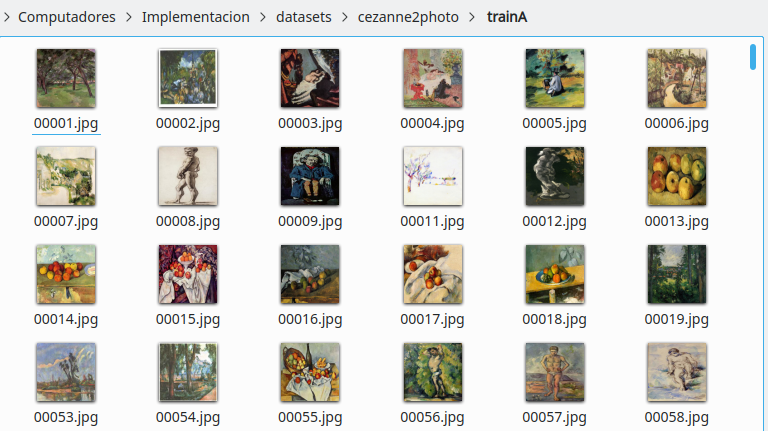
\includegraphics[width=1\textwidth]{imagenes/vista_previa_dataset_pintor.png}
    \caption{Vista previa de los cuadros}
    \label{fig:vista_previa_cuadros_cezanne}
  \end{subfigure}
  \hfill
  \begin{subfigure}[b]{0.49\textwidth}
    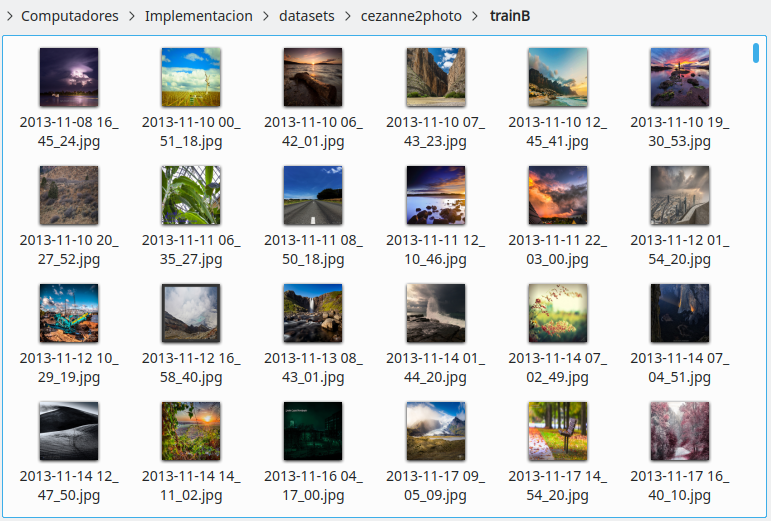
\includegraphics[width=1\textwidth]{imagenes/vista_previa_dataset_fotos.png}
    \caption{Vista previa de las fotografías}
    \label{fig:vista_previa_fotos_cezanne}
  \end{subfigure}
  \caption{Vista previa del dataset \textit{cezanne2photo}}
  \label{fig:vista_previa_cezanne_dataset}
\end{figure}


Por último, los autores crearon más datasets para su nueva arquitectura de red neuronal. Uno de sus autores, Taesung Park, los publicó en la url \url{https://people.eecs.berkeley.edu/~taesung_park/CycleGAN/datasets/}, dirección que utilizaremos en la implementación para descargarlos automáticamente. Asimismo, TensorFlow, en su herramienta de datasets, también los recoge para su uso.

\begin{figure}[h]
    \centering
    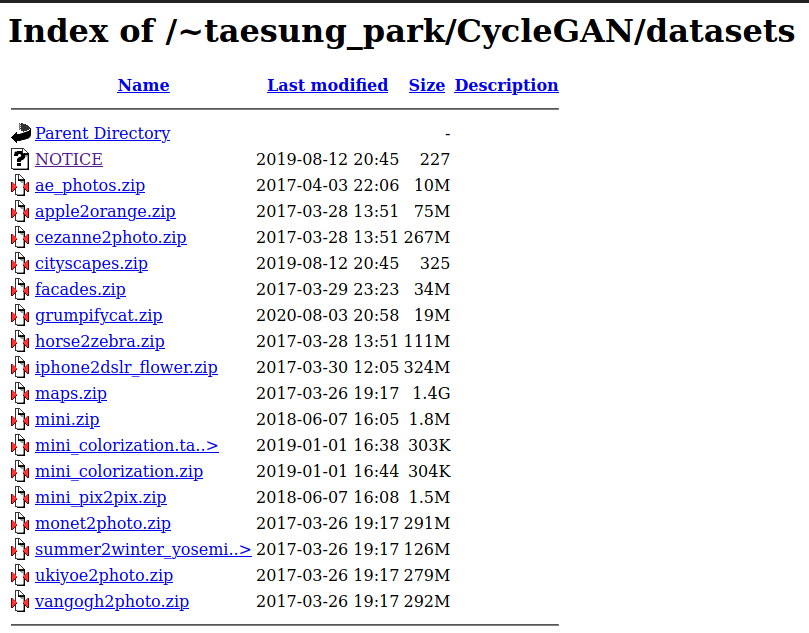
\includegraphics[width=0.7\textwidth]{imagenes/datasets_berkeley.png}
    \caption{Datasets creados por el equipo de Cycle GAN}
    \label{fig:datasets:berkeley}
\end{figure}

\section{Tecnologías utilizadas}
Dentro del mundo del Machine Learning existen numerosas herramientas de trabajo, siendo un entorno que se renueva a una velocidad de vértigo. \newline

El \textit{verano} que atraviesa la Inteligencia Artificial en general y la Visión Artificial en particular provocan que numerosas instituciones, empresas y particulares apuesten por desarrollar nuevas herramientas o mejorar las ya existentes. Algunos de esos contribuyentes son actores de la industria tan destacados como Google, Facebook y NVIDIA.
\newline

Por otra parte, en este Trabajo Final de Grado se han utilizado herramientas principalmente de código abierto y con amplia documentación, las cuales se detallan a continuación.
\subsection{Python}
Python es un lenguaje de programación que apareció en 1991, diseñado por Guido Van Rossum. Actualmente administrado por la Python Software Foundation y distribuido mediante una licencia de código abierto denominada Python Software Foundation License. \newline

En los últimos años ha ganado mucho peso en todos los ámbitos de la Informática, debido a su filosofía centrada en la legibilidad del código y su facilidad de aprendizaje. Sus características principales son las siguientes:
\begin{itemize}
  \item Soporta programación estructurada, orientada a objetos, imperativa y funcional, sin forzar al usuario a decantarse por ninguno de ellos y pudiendo cambiar entre ellos en cualquier momento. Este enfoque aúna las ventajas de cada paradigma, facilitando a los programadores utilizar la solución que deseen sin verse limitados por el lenguaje de programación.
  \item Posee un diseño que facilita la extensión del mismo y la interoperabilidad con otros lenguajes de programación, estimulando la creación de librerías y módulos compatibles con Python.
  \item A diferencia de otros lenguajes, su código es interpretado por un intérprete. Este enfoque proporciona un mayor soporte a la multiplaforma, existiendo implementaciones de Python escritas en lenguajes como C, Java o C\# para una gran cantidad de sistemas operativos.
  \item Proporciona un modo interactivo similar a una terminal de comandos, lo que permite un desarollo más cómodo para el programador al probar bloques de código independientemente de forma sencilla.
  \item Su sistema de tipos es fuertemente tipado y dinámico, lo que aporta una mayor seguridad en las operaciones del programa sin renunciar a facilitar el desarrollo y el mantenimiento del mismo.
  \item Incorpora soporte para la instalación de módulos mediante la herramienta pip, utilizada en este Trabajo Final de Grado para facilitar la instalación de las dependencias del sistema implementado.
\end{itemize}

\subsection{TensorFlow}
TensorFlow es una librería de cálculo numérico orientada a la computación distribuida, creada por Google y bajo el amparo de la licencia de código abierto Apache 2.0 desde noviembre de 2015.\newline 

Ha ganado mucho protagonismo en los últimos años ya que principalmente facilita el uso de tarjetas gráficas para acelerar la computación que necesitan los modelos de Machine Learning. Sus principales características son:
\begin{itemize}
    \item Permite variar el hardware de forma trasparente al programador, sin tener que realizar código adicional o transformarlo para las diferentes implementaciones. En otras palabras, implementa el Principio de inversión de dependencias, logrando que el programador dependa únicamente de abstracciones y no de los detalles de implementación.
    \item Internamente utiliza grafos de flujo de datos, lo que permite ciertas optimizaciones y un procesado vectorial de los propios datos, aumentando la eficiencia del software. Con la publicación de TensorFlow 2.0 el 30 de septiembre de 2019, no es necesario programar forzosamente mediante dichos grafos, permitiendo el uso de un paradigma imperativo (\textit{Eager Execution}) más intuitivo de cara al programador.
    \item Proporciona API para los siguientes lenguajes: Python (utilizada en este Trabajo Final de Grado), C++, Haskell, Java, Go y Rust.
\end{itemize}

\subsection{Tensorboard}
Tensorboard es la interfaz gráfica incluida con TensorFlow para facilitar la comprensión del software implementado. Posee herramientas para la visualización de gráficas asociadas a las métricas del modelo, lo que permite evaluar de forma rápida el proceso de aprendizaje del modelo ya que indica, además de la métrica, los metadatos que queramos además del tiempo transcurrido de ejecución. \newline

\begin{figure}[h!]
    \centering
    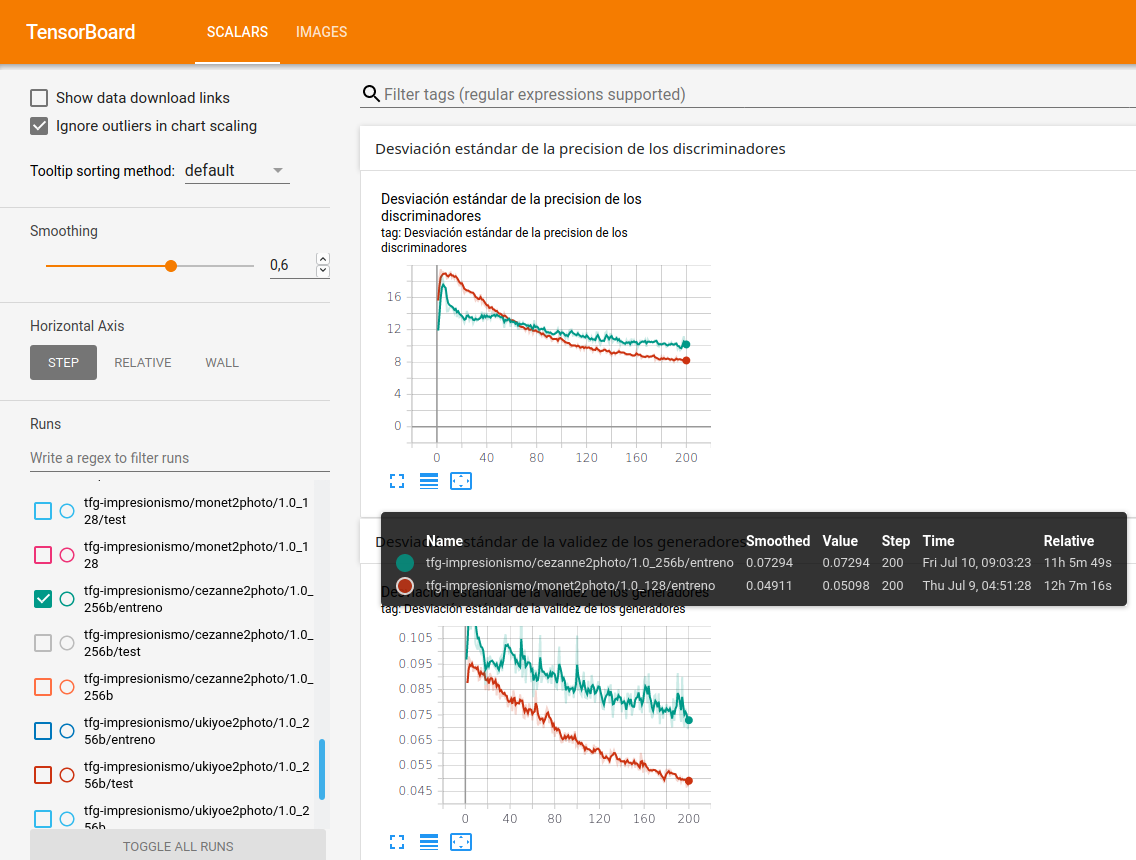
\includegraphics[width=0.75\textwidth]{imagenes/Tensorboard_graficas.png}
    \caption{Ejemplo de las gráficas proporcionadas por Tensorboard}
    \label{fig:tensorboard_descripcion_graficas}
\end{figure}

Asimismo dispone de opciones para visualizar imágenes relacionadas con el modelo, el grafo de computación ejecutado por TensorFlow, histogramas y distribuciones.

\begin{figure}[h!]
    \centering
    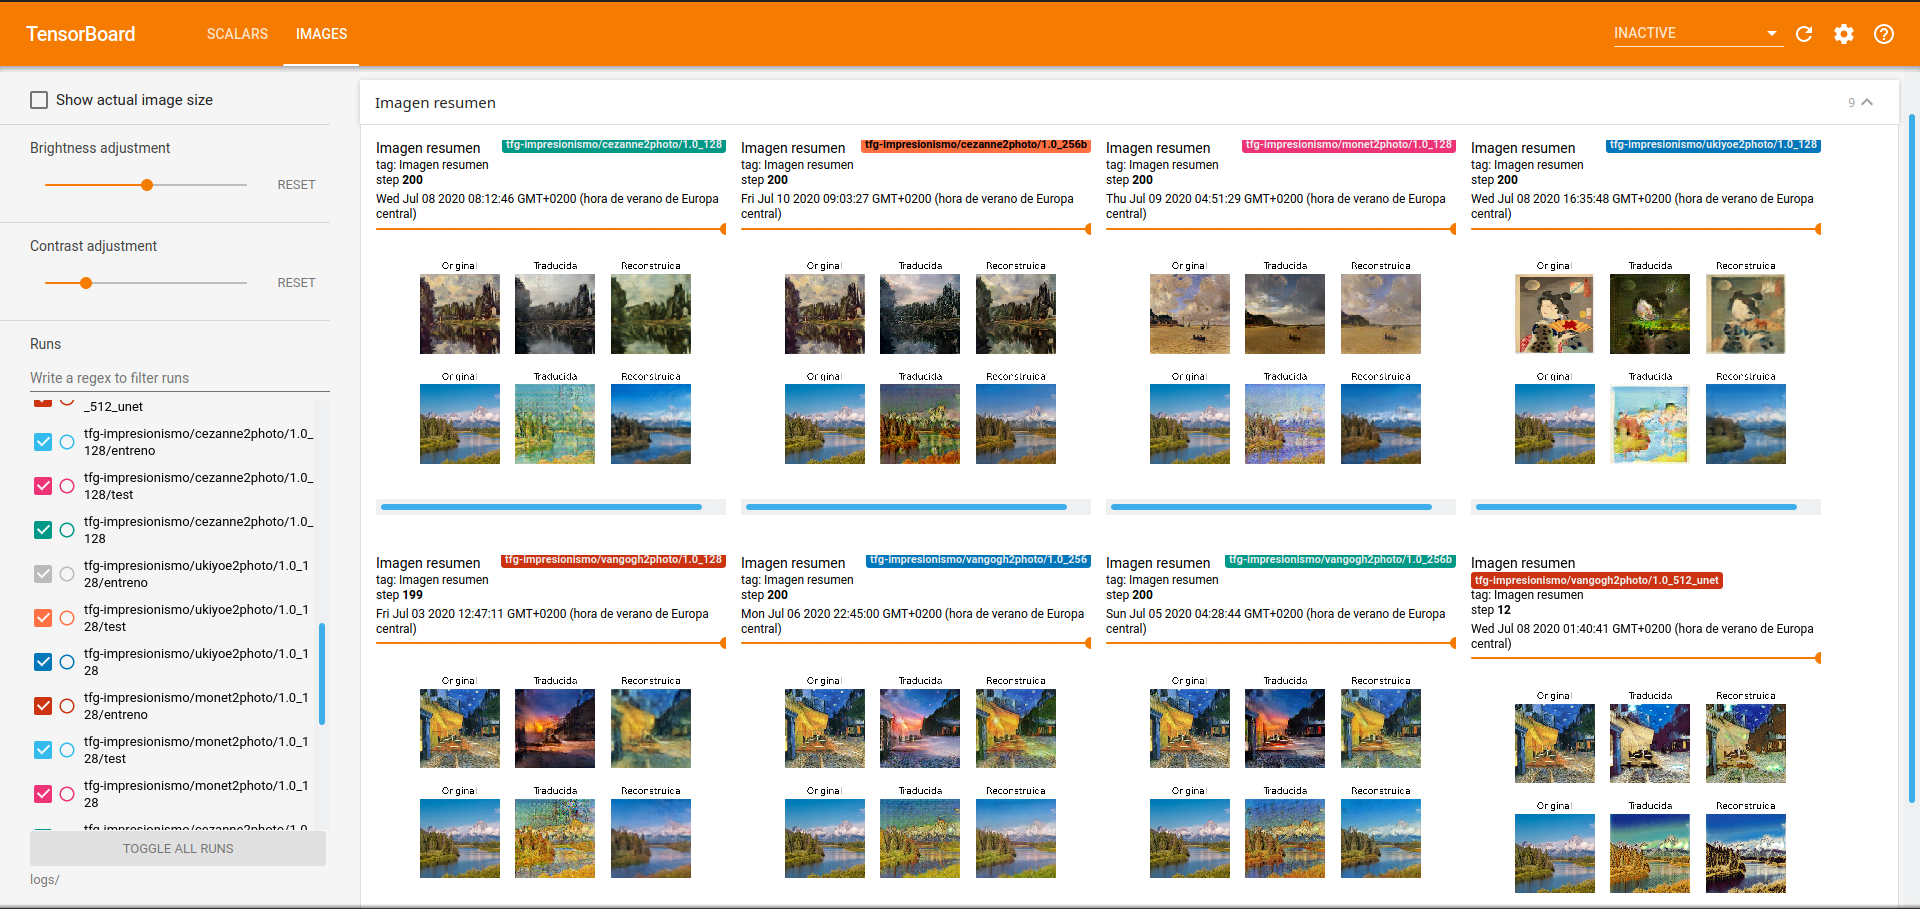
\includegraphics[width=1\textwidth]{imagenes/Tensorboard_imagen_resumen.png}
    \caption{Ejemplo de la visualización de fotos mediante Tensorboard}
    \label{fig:tensorboard_descripcion_imagenes}
\end{figure}

\subsection{Keras}
Keras es una API de Redes Neuronales que permite un desarrollo y mantenimiento cómodo y sencillo de las mismas. Desarrollada por François Chollet, fue lanzada el 27 de marzo de 2015 bajo la licencia de código abierto MIT. Dicha interfaz puede funcionar bajo TensorFlow, Theano y Microsoft Cognitive Toolkit, abstrayendo el modelo del \textit{background} computacional.
\newline

La combinación de TensorFlow con Keras es ampliamente utilizada en el sector debido a su sencillez de uso, potencia y eficacia. De hecho, TensorFlow en su versión 2 renunció a sus API de modelos predefinidos para ofrecer una integración completa y óptima con Keras.

\subsection{CUDA}

CUDA son las siglas de \textit{Compute Unified Device Architecture} (Arquitectura Unificada de Dispositivos de Cómputo), una plataforma para realizar procesamiento paralelo mediante las GPU de NVIDIA, creada en el año 2007. Esta herramienta permite utilizar las ventajas del paralelismo masivo que ofrecen las GPU mediante un dialecto de C, si bien existen enlaces para poder usarla desde Python, Fortran y MATLAB.
\newline

Con esta tecnología, podemos paralelizar de forma sencilla nuestras aplicaciones. Así mismo dispone de una extensión, llamada cuDNN, que optimiza las aplicaciones de Redes Neuronales, reduciendo aún más los tiempos de cómputo. De hecho, en este Trabajo Final de Grado es utilizada indirectamente, ya que es la plataforma que usa TensorFlow para paralelizar sus operaciones; si bien requiere una configuración un tanto problemática. Dicha situación se detallará en la sección \ref{sec:dependencias}

\subsection{Google Cloud Plataform}

Google Cloud Plataform es la plataforma de computación en la nube propiedad de Google, en la que se ofertan todo tipo de servicios. Mediante esta herramienta, los usuarios pueden contratar servicios de forma rápida y flexible, sujetos únicamente al pago por uso de los mismos. Entre otros, provee servicios de Inteligencia Artificial, Big Data y almacenamiento, además de máquinas virtuales totalmente configurables y de elevado rendimiento. \newline

\begin{figure}[h!]
    \centering
    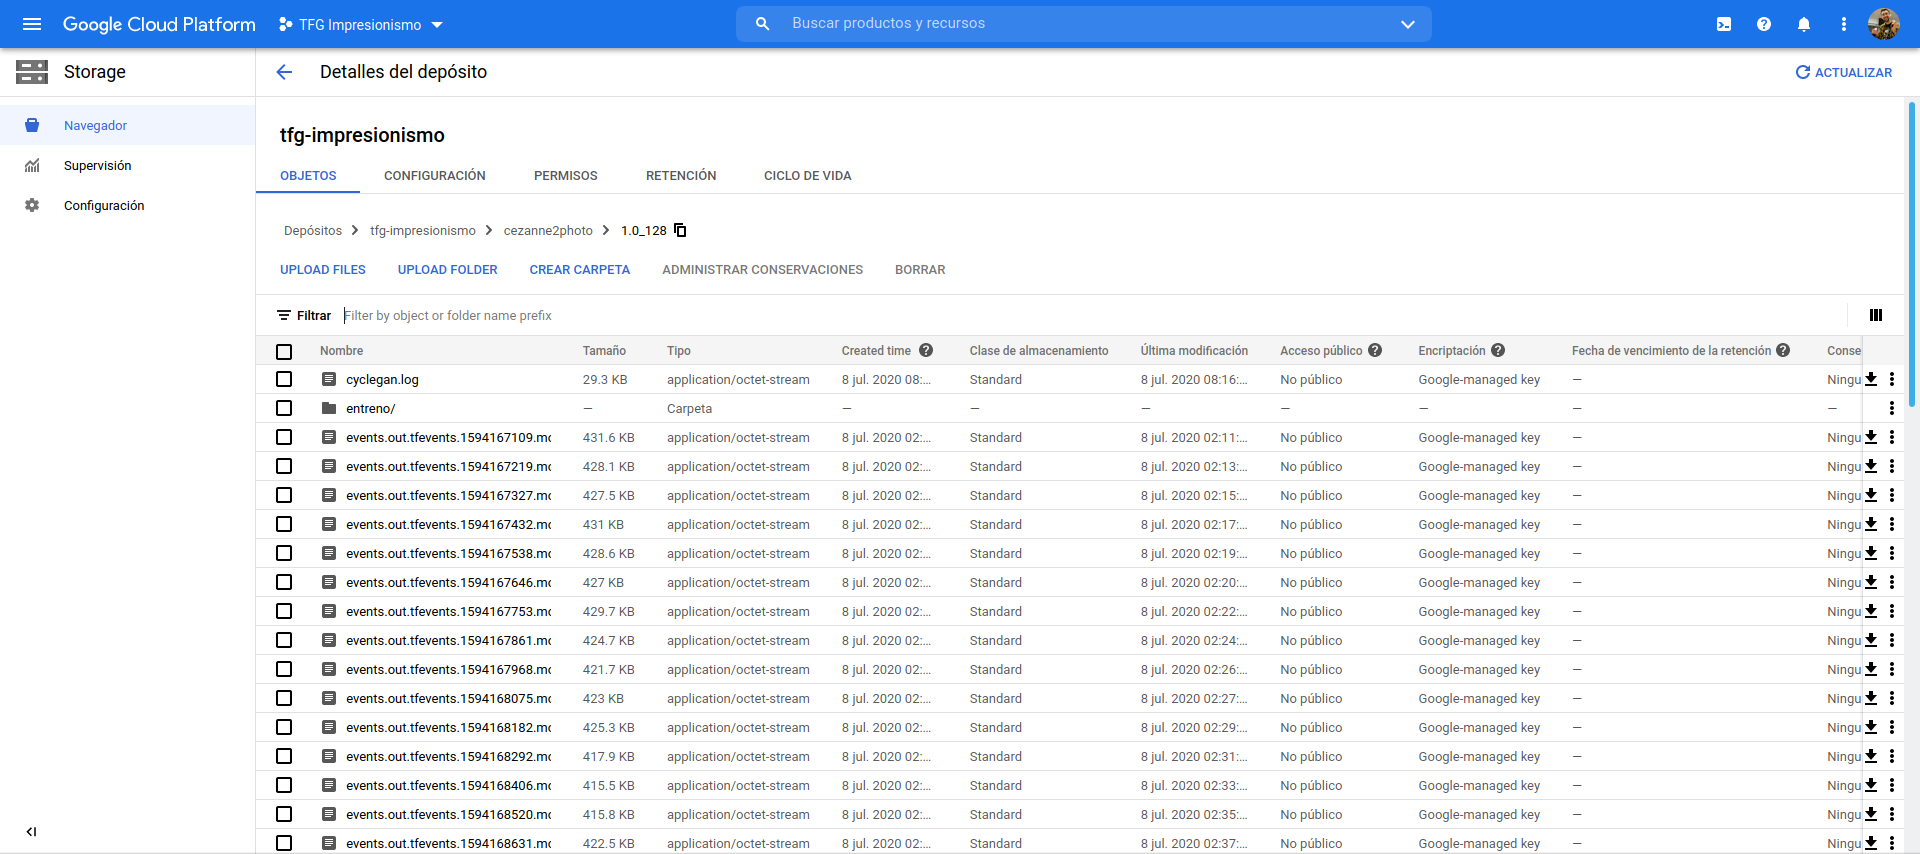
\includegraphics[width=1\textwidth]{imagenes/gcp_logs.png}
    \caption{Ejemplo de visualización de \textit{logs} de TensorBoard en el servicio de almacenamiento de Google Cloud Plataform}
    \label{fig:gcp_logs}
\end{figure}

En este Trabajo Final de Grado se ha utilizado esta plataforma para acceder a las GPU y TPU de Google, las cuales permiten acelerar en gran medida los tiempos de entrenamiento del sistema propuesto.

\begin{figure}[h!]
    \centering
    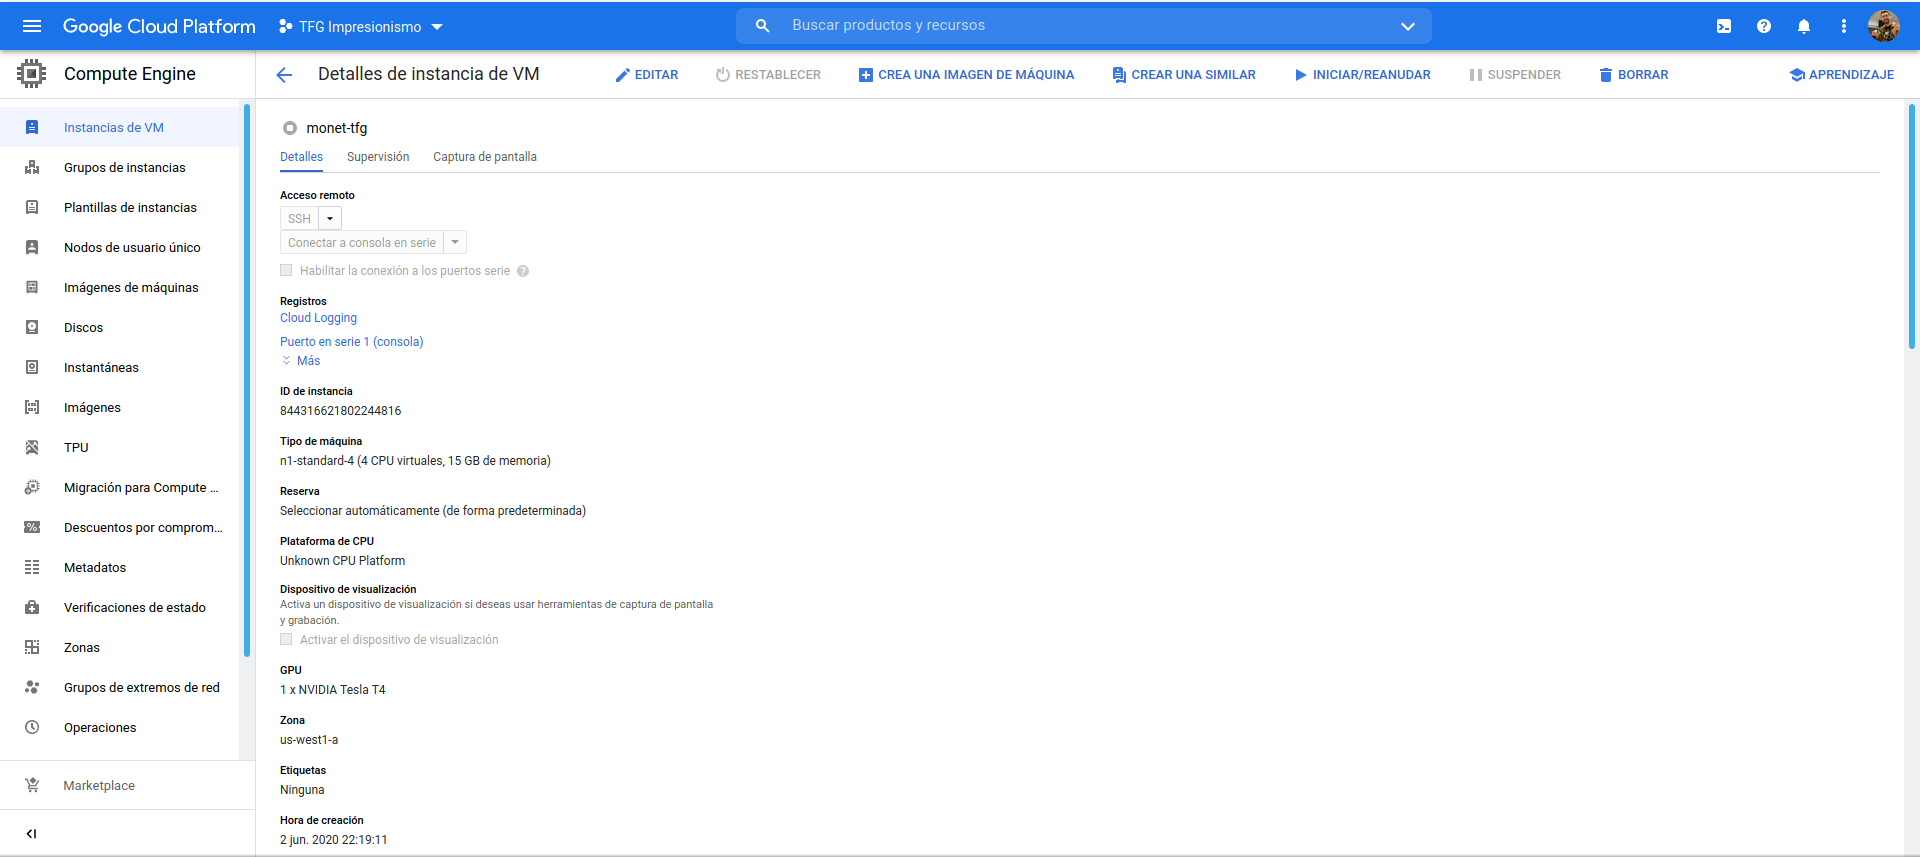
\includegraphics[width=1\textwidth]{imagenes/gcp_mv.png}
    \caption{Visualización de la descripción de la máquina virtual utilizada en este TFG alojada en Google Cloud Plataform}
    \label{fig:gcp_mv}
\end{figure}

\subsection{Flask}
Flask es un \textit{microframework} elaborado para desarrollo web mediante Python, creado por Armin Ronacher y liberado bajo la licencia de código abierto BSD. A diferencia de otros frameworks, Flask está pensado para crear aplicaciones web rápidamente, con una curva de aprendizaje suave para el programador; lo que permite desarrollar servicios de forma ágil y rápida.
\newline

Además añade soporte para la creación de API REST de forma extremadamente sencilla, que es el uso que le daremos en este Trabajo Final de Grado.

\subsection{Git y GitHub}

Git es un sistema de control de versiones \textit{open source} diseñado por Linus Torvalds (conocido por ser el artífice de Linux). Este sistema de control de versiones se caracteriza por su concepción distribuida, lo que permite prescindir de un servidor si así lo deseamos. Diseñado para el desarrollo no lineal de proyectos, fue desarrollado para la gestión del núcleo de Linux, lo que junto a su velocidad, eficiencia y facilidad de uso lo ha converido en uno de los sistemas más utilizados en todo el mundo. \newline

Por otra parte, GitHub es una plataforma propietaria diseñada principalmente para el alojamiento remoto de repositorios Git. Si bien no es necesaria para utilizar Git, ha adoptado una inmensa popularidad debido a que nos permite tener repositorios privados (ahorrando a los desarrolladores el despliegue y mantenimiento de un servidor) sin renunciar a crear repositorios públicos con los que compartir nuestro código hacia la comunidad. En este \tfg se ha utilizado tanto Git como GitHub para el control de versiones de la implementación \textit{software}.

\section{Diseño general del sistema}
\subsection{Sistema principal}

Este sistema es el núcleo del proyecto, ya que es el sistema que implementa la red Cycle GAN. En primer lugar expondremos la estructura de archivos del mismo, para posteriormente explicar las opciones de configuración, los casos de uso del sistema y por último la funcionalidad de todos los ficheros de código fuente.

\subsubsection{Estructura de archivos del sistema}

Se disponen de los siguientes directorios (además del archivo requirements.txt que es utilizado para la instalación de dependencias):

\begin{itemize}
    \item configuracion: contiene los archivos de configuración .json.
    \item datasets: recoge los conjuntos de imágenes a utilizar por el sistema (organizados por su nombre) para su entrenamiento y para la generación del conjunto test de resultados.
    \item input: dispone de las fotos que el usuario desee transformar a cuadros.
    \item logs: contiene los logs del sistema (según dataset y versión del sistema), tanto como los de depuración como los de TensorBoard.
        \begin{figure}[h!]
            \centering
            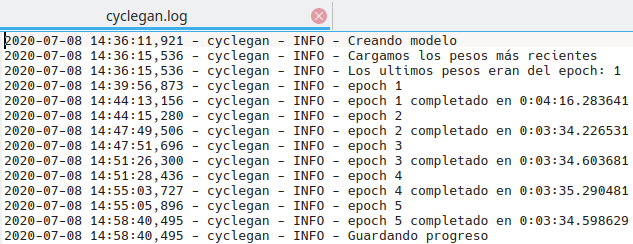
\includegraphics[width=1\textwidth]{imagenes/muestra_logs_cyclegan.png}
            \caption{Muestra de logs del sistema}
            \label{fig:muestra_logs_cyclegan}
        \end{figure}
    \item modelos: contiene los modelos que utiliza el sistema ya entrenados, organizados por dataset y versión. Dispone además de los \textit{checkpoints} de los propios modelos, guardados cada 5 epochs.
    \item output: recoge los resultados del sistema, organizados nuevamente por versión y dataset. Para cada uno de ellos dispone de las imágenes del usuario en la raíz, así como dos subdirectorios llamados test\textunderscore foto y test\textunderscore pintor, los cuales guardan los resultados finales sobre los conjuntos de test del dataset.
    \item src: dispone de los ficheros de código fuente.
\end{itemize}

\subsubsection{Configuración del sistema}

Tenemos dos secciones de configuración: los archivos .json y los parámetros de las lanzaderas del modelo.

    \paragraph{Archivos de configuración .json}
    Son leídos por el sistema al arrancar. Dispone de las siguientes secciones:
    \begin{itemize}
        \item configuración\textunderscore modelo: ajusta los parámetros del sistema, tales como la tasa de aprendizaje, las dimensiones de las imágenes, los epochs del entrenamiento y los filtros de los generadores y discriminadores, entre otras opciones.
        \item url: dispone de la url de la API del sistema ampliación de resolución (puede ser local o en línea) y de la url datasets, desde donde el sistema descarga los datasets en caso de no disponer de ellos.
        \item gcp: contiene la ruta del contenedor de Google Cloud Plataform donde almacenar los logs del sistema si se entrena en dicha plataforma.
        \item dataset: guarda, para cada dataset, las dos imágenes que se usan en la imagen resumen mostrada en tensorboard para seguir de forma gráfica el entrenamiento del sistema.
        \item varios: dispone de una opción, \textit{mascara\textunderscore logs}, que como su nombre indica es la máscara usada en el formateo de los logs del sistema.
    \end{itemize}
    
    La figura \ref{fig:ejemplo_json} indica un fichero json de ejemplo. El fichero que utilizemos debe contener, como mínimo, todos los campos mostrados de todas las secciones salvo de \textit{dataset}, en la que sólo se debe disponer de al menos un registro con los campos \textit{imagen\textunderscore pintor\textunderscore muestra} y \textit{imagen\textunderscore foto\textunderscore muestra}.
    
    \begin{figure}[h!]
            \centering
            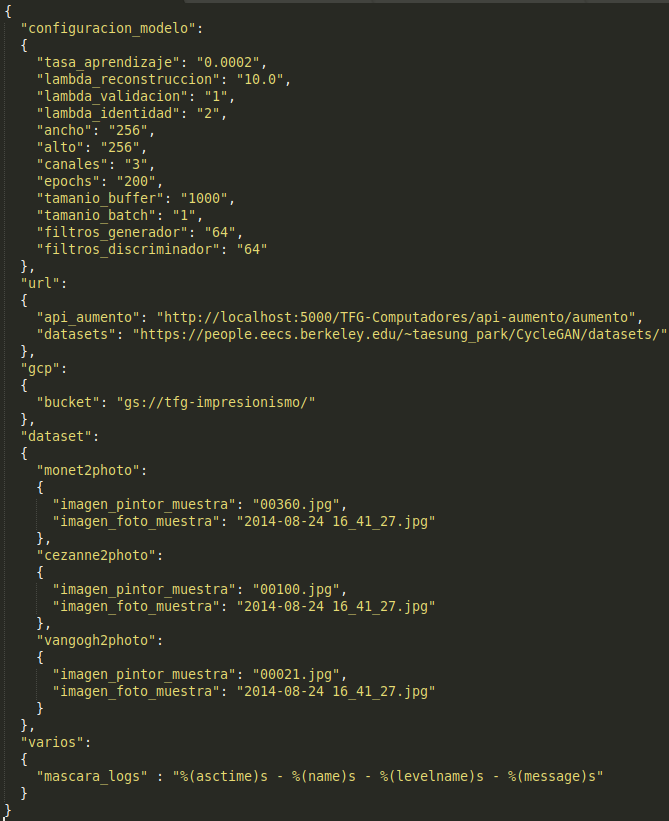
\includegraphics[width=1\textwidth]{imagenes/ejemplo_json.png}
            \caption{Ejemplo de archivo de configuración json}
            \label{fig:ejemplo_json}
    \end{figure}
    
    \paragraph{Opciones de las lanzaderas}
    Son las opciones relacionadas los ficheros lanzadera, explicados en las secciones \ref{seccion:entreno_sistema_cgan} y \ref{seccion:creacion_imagenes}. Dichas opciones se ajustan al invocar al sistema mediante la linea de comandos (o en las configuraciones si utilizamos un IDE), y son:
    \begin{itemize}
        \item versión (indicada con -v o --version): Especifica el nombre de la versión con la que se guardarán los archivos.
        \item dataset (expresada con -d o --dataset): Especifica el dataset a utilizar
        \item configuracion (indicada con -c o --configuracion): Indica el fichero de configuración .json a utilizar. Debe indicarse la extensión .json en el uso del mismo.
        \item arquitectura (expresada con -a o --arquitectura): Exclusiva de la lanzadera de entrenamiento, indica al sistema qué arquitectura del generador se debe de usar: u-net (unet) o ResNet (resnet).
    \end{itemize}

\subsubsection{Casos de uso}
Este sistema dispone de dos casos de uso, disponibles desde dos puntos de arranque (una para cada caso), llamadas lanzaderas, siendo una para el entrenamiento del sistema y otra para su puesta en marcha en la composición de cuadros (o producción).
    \paragraph{Entreno del sistema}
    \label{seccion:entreno_sistema_cgan}
    Si deseamos entrenar al sistema, debemos de ejecutar la lanzadera \textit{lanzadera\textunderscore entreno} con las opciones deseadas. Se asegura de que el fichero de configuración exista, que la arquitectura sea válida y que el dataset exista (descargándolo y extrayéndolo si no se dispone del mismo), para posteriormente crear la red, cargar el dataset y realizar el entrenamiento. Una vez dicho entrenamiento finaliza, serializa la red y finaliza la ejecución.
    \paragraph{Creación de imágenes}
    \label{seccion:creacion_imagenes}
    Sucede cuando invocamos la lanzadera \textit{lanzadera\textunderscore produccion}. Al igual que el caso anterior, comprueba que el fichero de configuración y el dataset existan, para posteriormente pintar las fotos indicadas en output y en datasets\textbackslash nombre correspondiente\textbackslash testB y \textit{fotografiar} los cuadros disponibles en en datasets\textbackslash nombre correspondiente\textbackslash testA; ignorando los resultados ya existentes.

\subsubsection{Ficheros de código fuente}
En esta sección se explica únicamente las labores que realiza cada módulo de código, no cada función concreta. Para observar las funciones en detalle, remitimos al anexo \ref{anexo:sistema_principal}

    \paragraph{ampliar\textunderscore imagen}
    Como el lector habrá supuesto, se encarga de ampliar la imagen que recibe de entrada. Esta función utiliza el sistema ampliador de resolución si está disponible (a través de una petición POST a la API del sistema, pasando la imagen como un string base64 y recibiendo un array de bytes), y en caso contrario amplia la imagen en un factor de aumento (recibido por parámetro).
    
    \paragraph{capas\textunderscore extra}
    Un módulo muy liviano, únicamente implementa una capa especial mediante una clase para la arquitectura ResNet, conocida como \textit{ReflectionPadding2D}.
    
    \paragraph{cargador\textunderscore imagenes}
    Define la clase CargadorImagenes, la cual alimenta de imágenes a la red en el proceso de entrenamiento de la misma encargándose de la lectura de las imágenes y su preprocesamiento. Asimismo, calcula los n\textunderscore batches que van a ejecutarse durante el entrenamiento. 
    
    \paragraph{cyclegan}
    Esta es la clase principal del sistema. Contiene la implementación de toda la red, incluyendo los generadores unet y ResNet. Se encarga de crear la red, entrenarla, cargar el último punto de guardado del entrenamiento si existe y de guardar la red cuando finaliza el entrenamiento para que pueda ser utilizada en la creación de cuadros. Por último, realiza la inferencia de imágenes (o transformación de cuadro a imagen y viceversa).
    
    \paragraph{lanzadera\textunderscore entreno}
    Arranca el sistema para el entrenamiento de la red, funcionalidad descrita en la sección \ref{seccion:entreno_sistema_cgan}.
    
    \paragraph{lanzadera\textunderscore produccion}
    Análogamente al caso anterior, inicializa el sistema para la inferencia de imágenes, funcionalidad descrita en la sección \ref{seccion:creacion_imagenes}.
    
    \paragraph{procesado\textunderscore imagenes}
    
    Dispone de funciones relacionadas con el procesado y transformaciones (tanto de tipos como de resolución) de imagen.
    
    \paragraph{singleton}
    Es un módulo muy sencillo, el cual contiene la definición del patrón de diseño singleton, el cual es usado por las clases CargadorImagenes y Utilidades.
    
    \paragraph{utilidades}
    Almacena todas las funciones útiles para el resto de clases: conversión de rutas de fichero, marcas de tiempo, existencia de \textit{gsutil} (herramienta de Google Cloud Platform para la gestión de sus contenedores de almacenamiento), copia de logs al contenedor de Google Cloud Platform, almacenamiento de rutas de ficheros, lectura del fichero de configuración...


\subsection{Sistema ampliador de resolución}
Este sistema, como su propio nombre indica, se encarga de realizar la ampliación de la resolución (en un factor de 4) utilizando la red GAN EnhanceNet. La implementación realizada en este \tfg se ha basado en la implementación oficial realizada por los propios autores en TensorFlow 1, adaptándola para su uso mediante una API REST. \newline

No obstante, se ha modificado el código de forma que puedan deshacerse los cambios y utilizarse de forma análoga al sistema principal. Esa versión alternativa se recoge en el repositorio de GitHub \url{https://github.com/VicDominguez/EnhanceNet-TFG/tree/91058eba0ebbcd1f126d441ec15ef3987a3caa5f}. \newline

Pasemos ahora a explicar el diseño de este sistema. A diferencia del anterior, este sistema no dispone de estructura de ficheros reseñable (únicamente contiene los ficheros de código, el archivo con los pesos de la red y el fichero requirements.txt de dependencias), ni de opciones de configuración. \newline

Asimismo, sólo disponemos de un caso de uso: recibir peticiones POST con una imagen adjunta (codificada en base64), realizar el aumento de resolución sobre la misma y devolver la imagen ampliada al cliente. \newline

Por último, expliquemos la funcionalidad de cada módulo de código fuente:
    \subsubsection{controlador\textunderscore modelo}
    Sirve de adaptador entre el modelo y las posibles ejecuciones del sistema (API REST, fichero imagen y fichero base64). En la implementación utilizada en este \tfg únicamente se utilizan las funciones relacionadas con la API REST.
    
    \subsubsection{modelo}
    Contiene la definición de la red EnhanceNet, así como la función inferencia, la cual crea la red, carga los pesos de la misma y ejecuta la ampliación de la misma.
    
    \subsubsection{principal}
    Despliega la API REST utilizando Flask. Se encarga de recibir la imagen a ampliar mediante peticiones POST, además de comprobar la integridad y el tipo de imagen.
    
    \subsubsection{procesado}
    Dispone de funciones para el procesamiento de la entrada y de la salida (tanto de fichero como de la API), además de encargarse del preprocesamiento de la imagen.
    
    \subsubsection{utils}
    Contiene funciones relacionadas con la gestión de rutas y constantes necesarias para el sistema.


Si se desea consultar el código de la implementación, remitimos al anexo \ref{anexo:sistema_ampliador}.

\section{Guía de uso}
\subsection{Instalación de dependencias}
\label{sec:dependencias}

Para ejecutar el código creado en este \tfg tenemos que satisfacer ciertas dependencias. En los primeros pasos las elecciones de versiones no son caprichosas, ya que este \tfg se ha programado principalmente bajo la versión 2.2.1 de TensorFlow (no impidiendo la ejecución de la versión 1.14 también utilizada). La figura \ref{fig:cuadro_versiones_tensorflow_cuda} muestra las versiones compatibles entre sí.

\begin{figure}[h!]
    \centering
    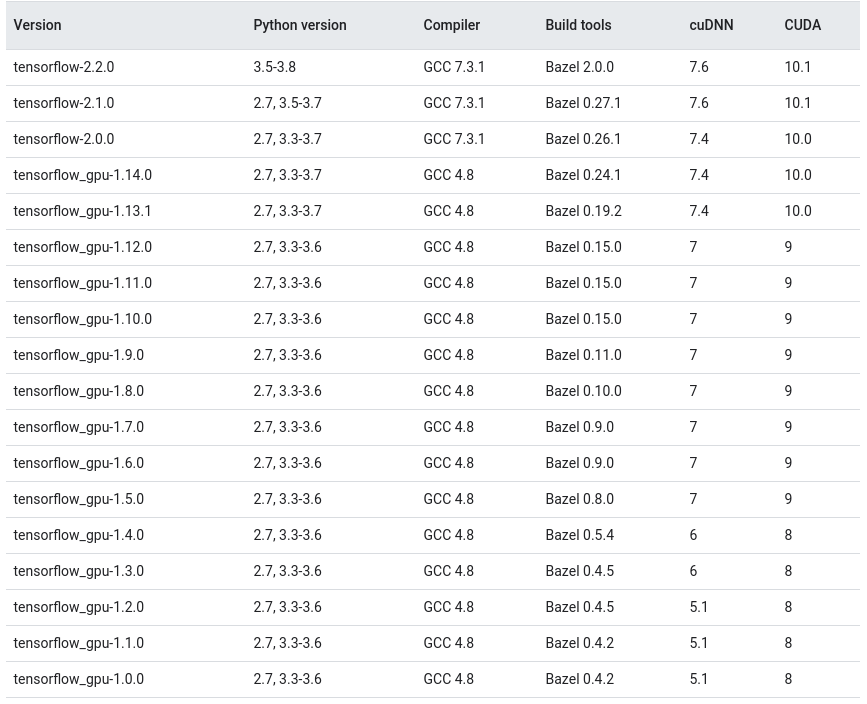
\includegraphics[width=1\textwidth]{imagenes/cuadro_versiones_tensorflow_cuda.png}
    \caption[Requisitos de versiones de NVIDIA de TensorFlow]{Requisitos de versiones de NVIDIA de TensorFlow. Extraído de \cite{StackOverflow2018}}
    \label{fig:cuadro_versiones_tensorflow_cuda}
\end{figure}

Enumeremos el proceso de instalación de las mismas:

\begin{enumerate}
    \item Disponer de una tarjeta gráfica NVIDIA en nuestro equipo que soporte (y si no lo tenemos, instalarlo)  como mínimo el driver 418.39 de la propia NVIDIA para poder instalar una versión CUDA igual o superior a 10.1. Se recomienda que disponga de al menos 2GB de VRAM para realizar la creación de cuadros.
    \item Instalaremos como mínimo CUDA 10.1 siguiendo el tutorial oficial de NVIDIA: \url{https://docs.nvidia.com/cuda/archive/10.1/index.html}
    \item Tras ello, instalamos la versión 7.6 para la versión de CUDA que hayamos instalado, siguiendo nuevamente el tutorial oficial \url{https://docs.nvidia.com/deeplearning/cudnn/install-guide/index.html}
    \item Si aún no lo tenemos instalado, descargamos el intérprete de Python y lo instalamos. Se recomienda utilizar un Entorno Integrado de Desarrollo (o IDE) como PyCharm.
    \item Si queremos ejecutar el sistema principal, necesitaremos tener instalado Git ya que es obligatorio para instalar dos dependencias concretas. Se puede instalar siguiendo la siguiente ayuda: \url{https://git-scm.com/book/en/v2/Getting-Started-Installing-Git}
    \item Instalamos el gestor de paquetes de Python pip siguiendo nuevamente el tutorial oficial: \url{https://pip.pypa.io/en/stable/installing/}
    \item Por último, según el subsistema que queramos ejecutar necesitaremos instalar las dependencias concretas del mismo. Si utilizamos un IDE como PyCharm el propio programa nos ayuda a instalarlas. Si no es ese caso, podemos instalarlas mediante el siguiente comando: \mint{bash}|pip3 install -r requirements.txt| 
\end{enumerate}

\subsection{Creación de cuadros}

La creación de cuadros es extremadamente sencilla: en la carpeta input situaremos nuestras imágenes, como se ilustra en la figura \ref{fig:muestra_input}.

\begin{figure}[h!]
    \centering
    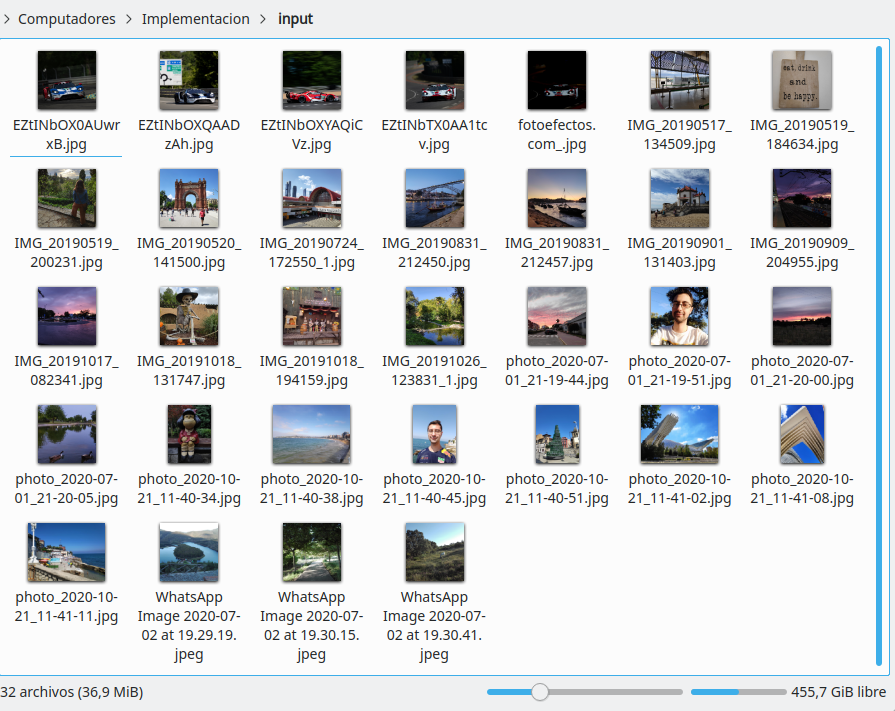
\includegraphics[width=0.75\textwidth]{imagenes/muestra_input.png}
    \caption{Ejemplo de contenido input}
    \label{fig:muestra_input}
\end{figure}

Tras ello, ejecutamos el sistema mediante el acceso \textit{lanzadera\textunderscore producción} (y con el subsistema de ampliación ejecutándose si así lo deseamos). Accedemos a la carpeta output \textgreater nombre de nuestro dataset \textgreater nombre de nuestra versión (campo -v de \textit{lanzadera\textunderscore producción}) y ahí están nuestros cuadros, tal como refleja la figura \ref{fig:muestra_output}

\begin{figure}[h!]
    \centering
    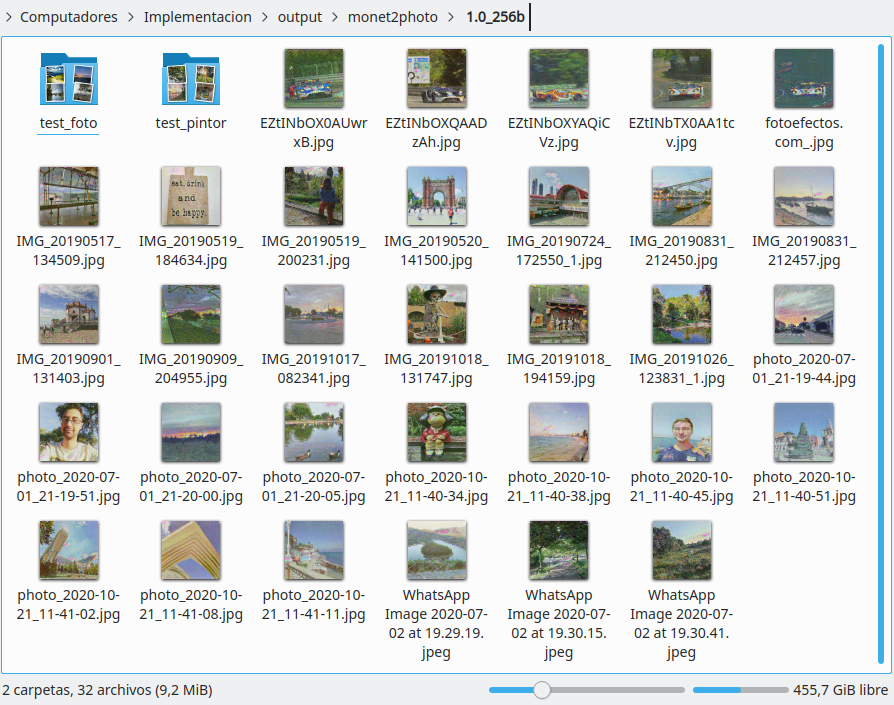
\includegraphics[width=0.75\textwidth]{imagenes/muestra_output.png}
    \caption{Ejemplo de cuadros generados}
    \label{fig:muestra_output}
\end{figure}

\subsection{Creación de modelos personalizados}

En este aspecto tenemos que distinguir varios casos:

\begin{itemize}
    \item Si queremos modificar los parámetros del modelo, únicamente tenemos que crear o modificar un fichero .json de configuración y editar los valores deseados de los campos de la sección \textit{configuracion\textunderscore modelo}. No olvidar indicar a la lanzadera el fichero de configuración a utilizar.
    \item Si deseamos entrenar al sistema con otros datos, tenemos dos supuestos: 
    
    \begin{enumerate}
        \item Si queremos utilizar un dataset recogido en la figura \ref{fig:datasets:berkeley}, tenemos que indicarlo en el campo -d de la lanzadera y recoger en el fichero .json de configuración una entrada similar a la indicada en la sección \textit{dataset}; como se muestra en la figura \ref{fig:parametros_dataset_berkeley}. 
        
            \begin{figure}[h!]
            \centering
            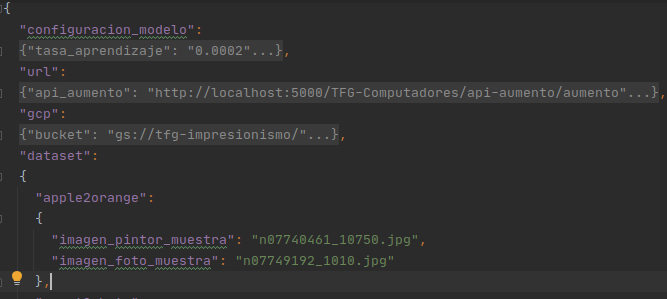
\includegraphics[width=0.75\textwidth]{imagenes/parametros_nuevo_dataset_berkeley.png}
            \caption{Parámetros para un nuevo dataset}
            \label{fig:parametros_dataset_berkeley}
            \end{figure}
        
        \item Si queremos crear un nuevo dataset (por ejemplo, uniendo los datasets monet2photo, cezanne2photo y vangogh2photo), además de realizar el procedimiento del caso anterior, a la hora de crear el dataset tenemos que respetar la estructura en carpetas \textit{trainA}, \textit{trainB}, \textit{testA} y \textit{testB} (todas ellas guardadas en el mismo directorio). \newline
        Posteriormente debemos bien guardar dichas carpetas en el directorio datasets del sistema o comprimir dichas carpetas en un único archivo de extensión zip y subirlas a una url. Dicha dirección se la indicamos al archivo de configuración en el campo \textit{datasets} de la sección \textit{url}, como se indica en la ilustración \ref{fig:url_json}.
            \begin{figure}[h!]
            \centering
            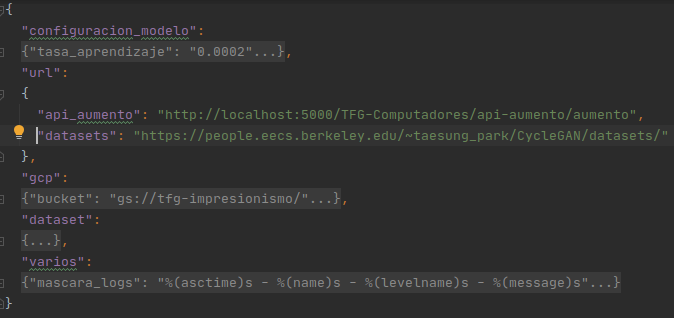
\includegraphics[width=0.75\textwidth]{imagenes/url_json.png}
            \caption{Parámetro url para un nuevo dataset}
            \label{fig:url_json}
            \end{figure}
        
        \end{enumerate}
\end{itemize}



\end{document}